\begin{frame}%[plain, noframenumbering, t]
    \frametitle{Проблемная ситуация}

    При создании прикладного ПО для специализированного аппаратного обеспечения
    дорого обеспечивать разработчиков самим аппаратным обеспечением.

    \textbf{Причины сложившейся ситуации:}
    \begin{itemize}
        \item призводство экземпляров аппаратного обеспечения в условиях санкций и дефицита полупроводников стала дорогой;
        \item простаивание программистов, пока происходит призводство и доставка аппаратного обеспечения;
        \item трудоемкость создания собственного виртуального аппаратного обеспечения.
    \end{itemize}
\end{frame}


\begin{frame}%[plain, noframenumbering, t]
    \frametitle{Пример специализированного аппаратного обеспечения}
    \begin{figure}[!htbp]
        \centering
        \begin{adjustbox}{max totalsize={0.8\textwidth}{0.8\textheight}}
            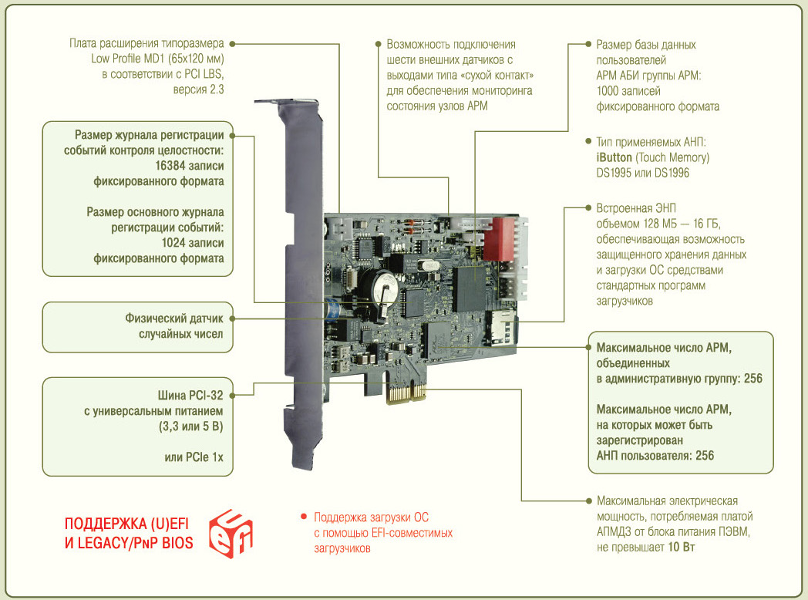
\includegraphics[]{images/apmdz.png}
        \end{adjustbox}
        \caption{Аппаратно-программный модуль доверенной загрузки Максим-М1}
    \end{figure}
\end{frame}


\begin{frame}%[plain, noframenumbering, t]
    \frametitle{Цель и задачи диссертации}
    \textbf{Цель:} снижение трудоемкости создания виртуальных устройств.

    \textbf{Задачи:}
    \begin{itemize}
        \item аналитический обзор существующих методов создания виртуального аппаратного обеспечения;
        \item формализация задачи создания виртуального аппаратного обеспечения;
        \item создание методики и алгоритма генерации виртуального аппаратного обеспечения на основе его спецификации;
        \item разработка лингвистического аппарата (семантика, синтаксис) языка для создания программ по генерации виртуального
            аппаратного обеспечения;
        \item выбор метрики оценки эффективности и оценка эффективности.
    \end{itemize}
\end{frame}


\begin{frame}%[plain, noframenumbering, t]
    \frametitle{Положения, выносимые на защиту}
    \begin{itemize}
        \item формализация задачи создания виртуального аппаратного обеспечения;
        \item формализованное представление алгоритма генерации виртуального аппаратного обеспечения;
        \item формализованное представление методики генерации виртуального аппаратного обеспечения;
        \item лингвистический аппарат (синтаксис, семантика) языка для создания программ по генерации виртуального
            аппаратного обеспечения;
        \item метрики оценки эффективности;
        \item экспериментальные результаты применения генератора аппаратного обеспечения.
    \end{itemize}
\end{frame}


\begin{frame}%[plain, noframenumbering, t]
    \frametitle{Анализ существующих методов создания виртуального аппаратного обеспечения}
    \newcommand{\tabitem}{{\textbullet}~}
        {\footnotesize
            \begin{longtable}{| p{3cm} | p{3cm} | p{4cm} |}
                \hline
                Метод & Особенности & Недостатки \\
                \hline
                    Создание stub-симулятора &
                    Требует создания интерфейсов-адапторов в прикладном ПО &
                    Приходится создавать интерфейсы-адапторы для каждого разрабатываемого ПО \\
                \hline
                    Использование записи работы аппаратного обеспечения &
                    Быстрый метод, не требует специальных знаний о внутреннем устройстве аппаратного обеспечения &
                    \tabitem Взаимодействие ПО с аппаратным обеспечением ограничивается заранее записанными сценариями \\
                \makecell{} & \makecell{} & \tabitem Количество записей очень быстро разрастается \\
                \makecell{} & \makecell{} & \tabitem Зачастую записи снимаются только с корректных сценариев использования \\
                \hline
                Использование эмулятора QEMU &
                \tabitem Готовая инфраструктура для создания виртуального аппаратного обеспечения &
                \tabitem Необходимость написания виртуального аппаратного обеспечения на низкоуровневом языке \\
                \makecell{} &
                \tabitem Постоянная поддержка эмулятора силами сообщества &
                \tabitem Необходимость обучения объектной системе QEMU (QOM) \\
                \hline
            \end{longtable}
        }
\end{frame}


\begin{frame}%[plain, noframenumbering, t]
    \frametitle{Объектная модель QEMU (QOM)}
    \begin{figure}[!htbp]
        \scalebox{0.075}{
            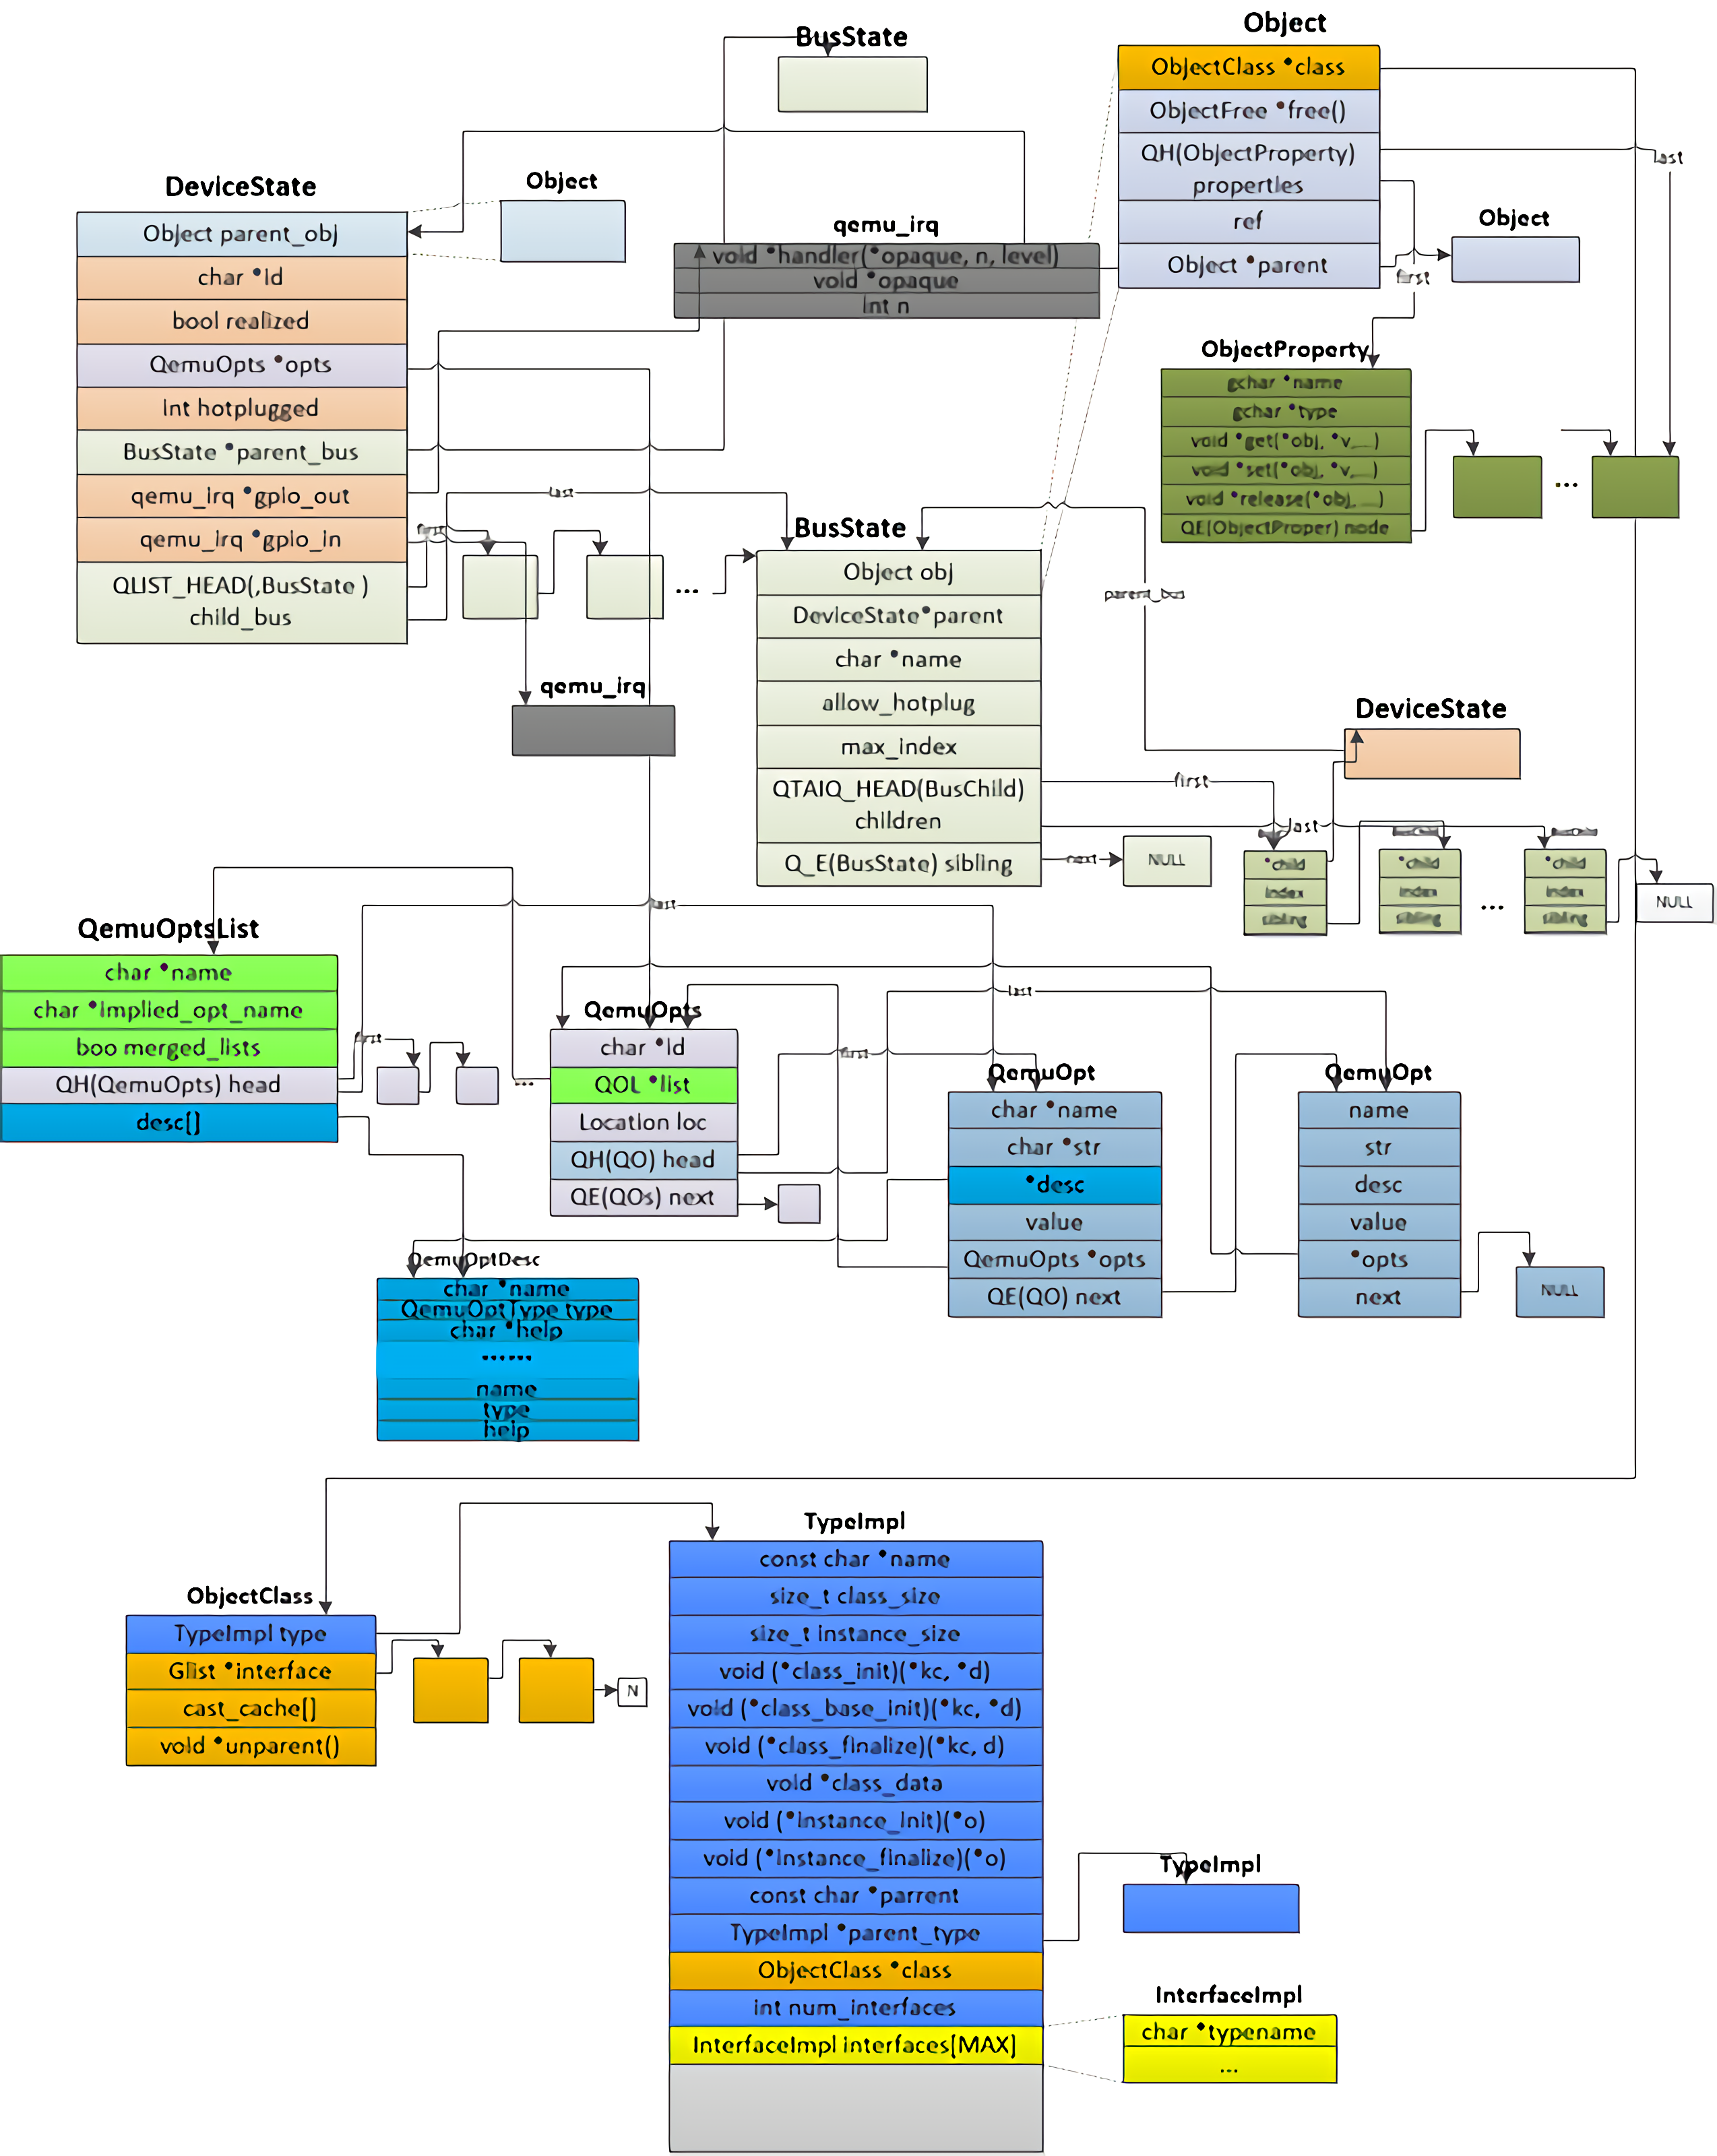
\includegraphics[]{images/qom-hierarchy_upscaled.png}
        }
    \end{figure}
\end{frame}


\begin{frame}%[plain, noframenumbering, t]
    \frametitle{Формализация задачи создания виртуального аппаратного обеспечения}
    Время разработки виртуального аппаратного обеспечения
    можно выразить формулой $T = L + D + C + R$, где
    \begin{itemize}
        \item $L$ -- время анализа QOM для реализации виртуального аппаратного обеспечения;
        \item $D$ -- описание устройства в терминах QOM;
        \item $C$ -- программирование логики устройства;
        \item $R$ -- тестирование и отладка.
    \end{itemize}

    Порог вхождения в QOM для программиста высок, из-за чего
    $L + D > C + R$.
    В данном исследовании стоит задача уменьшения $L$ и $D$,
    для уменьшения общего времени разработки виртуального аппаратного
    обеспечения.
\end{frame}


\begin{frame}%[plain, noframenumbering, t]
    \frametitle{Формализация задачи создания виртуального аппаратного обеспечения}
    Пусть задан ориентированный взвешенный граф $G = (V,E)$,
    где $V$ -- множество вершин графа, являющимися коммитами
    в системе контроля версий, а $E$ -- множество ребер.

    Весом ребра является время, затраченное программистом на
    формирование коммита. Общее время, затраченное на
    формирование цепочки коммитов можно рассчитать по
    формуле:

    $\sum_{i=1}^{n} f(e_{i,i+1})$, где $f$ -- весовая функция
    отображающая ребра в их веса: $f : E \rightarrow \mathbb{R}$
\end{frame}


\begin{frame}%[plain, noframenumbering, t]
    \frametitle{Методика создания виртуального аппаратного обеспечения}
    \begin{figure}[!htbp]
        \hspace*{-5cm}
        \scalebox{0.7}{
            % !TEX encoding = UTF-8 Unicode
% Úτƒ-8 encoded
% http://www.linux.org.ru/forum/general/10357036
\tikzset{
    line/.style={draw, -latex'},
    every join/.style={line},
    u/.style={anchor=south},
    r/.style={anchor=west},
    fxd/.style={text width = 6em},
    it/.style={font={\small\itshape}},
    bf/.style={font={\small\bfseries}},
}
\tikzstyle{base_long} =
    [
        draw,
        on chain,
        on grid,
        align=center,
        minimum height=4ex,
        minimum width = 10ex,
        node distance = 6mm and 60mm,
        text badly centered,
    ]
\tikzstyle{base} =
    [
        draw,
        on chain,
        on grid,
        align=center,
        minimum height=4ex,
        minimum width = 10ex,
        node distance = 6mm and 60mm,
        text badly centered,
        text width=5cm
    ]
\tikzstyle{coord} =
    [
        coordinate,
        on chain,
        on grid
    ]
\tikzstyle{cloud} =
    [
        base,
        ellipse,
        node distance = 3cm,
        minimum height = 2em,
        text width=2cm
    ]
\tikzstyle{decision} =
    [
        base,
        diamond,
        aspect=2,
        node distance = 2cm,
        inner sep = 0pt
    ]
\tikzstyle{block} =
    [
        rectangle,
        base,
        rounded corners,
        minimum height = 2em
    ]
\tikzstyle{print_block} =
    [
        base,
        tape,
        tape bend top=none,
    ]
\tikzstyle{io} =
    [
        base,
        trapezium,
        trapezium left angle = 70,
        trapezium right angle = 110,
    ]
\tikzstyle{prompt} =
    [
        base,
        trapezium,
        trapezium left angle = 90,
        trapezium right angle = 80,
        shape border rotate = 90
    ]
\tikzstyle{disk file} =
    [
        base,
        cylinder,
        aspect=0.2,
    ]
\tikzstyle{process} =
    [
        rectangle,
        base,
    ]
\makeatletter
\pgfkeys{/pgf/.cd,
    subrtshape w/.initial=2mm,
    cycleshape w/.initial=2mm
}
\pgfdeclareshape{parallelshape}{
    \inheritsavedanchors[from=rectangle]
    \inheritanchorborder[from=rectangle]
    \inheritanchor[from=rectangle]{north}
    \inheritanchor[from=rectangle]{center}
    \inheritanchor[from=rectangle]{west}
    \inheritanchor[from=rectangle]{east}
    \inheritanchor[from=rectangle]{mid}
    \inheritanchor[from=rectangle]{base}
    \inheritanchor[from=rectangle]{south}
    \backgroundpath{
        \southwest \pgf@xa=\pgf@x \pgf@ya=\pgf@y
        \northeast \pgf@xb=\pgf@x \pgf@yb=\pgf@y
        \def\ppd@offset{\pgfpoint{\pgfutil@tempdima}{0ex}}
        \def\ppd@offsetm{\pgfpoint{-\pgfutil@tempdima}{0ex}}
        \pgfpathmoveto{\pgfqpoint{\pgf@xa}{\pgf@ya}}
            \pgfpathlineto{\pgfqpoint{\pgf@xb}{\pgf@ya}}
        \pgfpathclose
        \pgfpathmoveto{\pgfqpoint{\pgf@xb}{\pgf@yb}}
            \pgfpathlineto{\pgfqpoint{\pgf@xa}{\pgf@yb}}
        \pgfpathclose
    }
}
\pgfdeclareshape{subrtshape}{
    \inheritsavedanchors[from=rectangle]
    \inheritanchorborder[from=rectangle]
    \inheritanchor[from=rectangle]{north}
    \inheritanchor[from=rectangle]{center}
    \inheritanchor[from=rectangle]{west}
    \inheritanchor[from=rectangle]{east}
    \inheritanchor[from=rectangle]{mid}
    \inheritanchor[from=rectangle]{base}
    \inheritanchor[from=rectangle]{south}
    \backgroundpath{
        \southwest \pgf@xa=\pgf@x \pgf@ya=\pgf@y
        \northeast \pgf@xb=\pgf@x \pgf@yb=\pgf@y
        \pgfmathsetlength\pgfutil@tempdima{\pgfkeysvalueof{/pgf/subrtshape w}}
        \def\ppd@offset{\pgfpoint{\pgfutil@tempdima}{0ex}}
        \def\ppd@offsetm{\pgfpoint{-\pgfutil@tempdima}{0ex}}
        \pgfpathmoveto{\pgfqpoint{\pgf@xa}{\pgf@ya}}
        \pgfpathlineto{\pgfqpoint{\pgf@xb}{\pgf@ya}}
        \pgfpathlineto{\pgfqpoint{\pgf@xb}{\pgf@yb}}
        \pgfpathlineto{\pgfqpoint{\pgf@xa}{\pgf@yb}}
        \pgfpathclose
        \pgfpathmoveto{\pgfpointadd{\pgfpoint{\pgf@xa}{\pgf@yb}}{\ppd@offsetm}}
        \pgfpathlineto{\pgfpointadd{\pgfpoint{\pgf@xa}{\pgf@ya}}{\ppd@offsetm}}
        \pgfpathlineto{\pgfpointadd{\pgfpoint{\pgf@xb}{\pgf@ya}}{\ppd@offset}}
        \pgfpathlineto{\pgfpointadd{\pgfpoint{\pgf@xb}{\pgf@yb}}{\ppd@offset}}
        \pgfpathclose
    }
}
\pgfdeclareshape{cyclebegshape}{
    \inheritsavedanchors[from=rectangle]
    \inheritanchorborder[from=rectangle]
    \inheritanchor[from=rectangle]{north}
    \inheritanchor[from=rectangle]{center}
    \inheritanchor[from=rectangle]{west}
    \inheritanchor[from=rectangle]{east}
    \inheritanchor[from=rectangle]{mid}
    \inheritanchor[from=rectangle]{base}
    \inheritanchor[from=rectangle]{south}
    \backgroundpath{
        \southwest \pgf@xa=\pgf@x \pgf@ya=\pgf@y
        \northeast \pgf@xb=\pgf@x \pgf@yb=\pgf@y
        \pgfmathsetlength\pgfutil@tempdima{\pgfkeysvalueof{/pgf/cycleshape w}}
        \pgfpathmoveto{\pgfqpoint{\pgf@xa}{\pgf@ya}}
\pgfpathlineto{\pgfpointadd{\pgfpoint{\pgf@xa}{\pgf@yb}}{\pgfpoint{0ex}{-\pgfutil@tempdima}}}
\pgfpathlineto{\pgfpointadd{\pgfpoint{\pgf@xa}{\pgf@yb}}{\pgfpoint{\pgfutil@tempdima}{0ex}}}
\pgfpathlineto{\pgfpointadd{\pgfpoint{\pgf@xb}{\pgf@yb}}{\pgfpoint{-\pgfutil@tempdima}{0ex}}}
\pgfpathlineto{\pgfpointadd{\pgfpoint{\pgf@xb}{\pgf@yb}}{\pgfpoint{0ex}{-\pgfutil@tempdima}}}
\pgfpathlineto{\pgfqpoint{\pgf@xb}{\pgf@ya}}
        \pgfpathclose
    }
}
\pgfdeclareshape{cycleendshape}{
    \inheritsavedanchors[from=rectangle]
    \inheritanchorborder[from=rectangle]
    \inheritanchor[from=rectangle]{north}
    \inheritanchor[from=rectangle]{center}
    \inheritanchor[from=rectangle]{west}
    \inheritanchor[from=rectangle]{east}
    \inheritanchor[from=rectangle]{mid}
    \inheritanchor[from=rectangle]{base}
    \inheritanchor[from=rectangle]{south}
    \backgroundpath{
        \southwest \pgf@xa=\pgf@x \pgf@ya=\pgf@y
        \northeast \pgf@xb=\pgf@x \pgf@yb=\pgf@y
        \pgfmathsetlength\pgfutil@tempdima{\pgfkeysvalueof{/pgf/cycleshape w}}
        \pgfpathmoveto{\pgfqpoint{\pgf@xb}{\pgf@yb}}
\pgfpathlineto{\pgfpointadd{\pgfpoint{\pgf@xb}{\pgf@ya}}{\pgfpoint{0ex}{\pgfutil@tempdima}}}
\pgfpathlineto{\pgfpointadd{\pgfpoint{\pgf@xb}{\pgf@ya}}{\pgfpoint{-\pgfutil@tempdima}{0ex}}}
\pgfpathlineto{\pgfpointadd{\pgfpoint{\pgf@xa}{\pgf@ya}}{\pgfpoint{\pgfutil@tempdima}{0ex}}}
\pgfpathlineto{\pgfpointadd{\pgfpoint{\pgf@xa}{\pgf@ya}}{\pgfpoint{0ex}{\pgfutil@tempdima}}}
\pgfpathlineto{\pgfqpoint{\pgf@xa}{\pgf@yb}}
        \pgfpathclose
    }
}
\makeatother
\tikzstyle{subroutine} =
    [
        base,
        subrtshape,
    ]
\tikzstyle{cyclebegin} =
    [
        base,
        cyclebegshape,
    ]
\tikzstyle{cycleend} =
    [
        base,
        cycleendshape,
    ]
\tikzstyle{connector} =
    [
        base,
        circle,
    ]

\tikzstyle{parallel} =
    [
        base_long,
        parallelshape,
    ]
\begin{tikzpicture}[%
    start chain=going below,    % General flow is top-to-bottom
    node distance=6mm and 30mm, % Global setup of box spacing
    ]
        \node  [] (classic)
                {Классическая методика};

        \node  [rectangle,
                base,
                minimum width=6cm] (analysis)
                [below = 3cm of classic]
                {Анализ QOM для реализации определенного аппаратного обеспечения};

        \node  [rectangle,
                base,
                minimum width=6cm] (QOM desc)
                [below = 4cm of analysis]
                {Описание аппаратного обеспечения в терминах QOM};

        \node  [rectangle,
                base,
                minimum width=6cm] (device logic)
                [below = 4cm of QOM desc]
                {Написание логики аппаратного обеспечения};

        \node  [rectangle,
                base,
                minimum width=6cm] (build config)
                [below = 4cm of device logic]
                {Встраивание виртуального аппаратного обеспечения в сборку QEMU};

        \node  [rectangle,
                base,
                minimum width=6cm] (compilation)
                [below = 4cm of build config]
                {Компиляция QEMU};

        \draw [->] (analysis) -- (QOM desc);
        \draw [->] (QOM desc) -- (device logic);
        \draw [->] (device logic) -- (build config);
        \draw [->] (build config) -- (compilation);

        %------

        \node  [] (modern)
                [right = 3cm of classic]
                {Разработанная методика};

        \node  [rectangle,
                base,
                minimum width=6cm] (modern analysis)
                [below = 3cm of modern]
                {Выбор устройства QEMU для наследования};

        \node  [rectangle,
                base,
                minimum width=6cm] (modern lang)
                [below = 4cm of modern analysis]
                {Описание устройства на разработаном языке};

        \node  [rectangle,
                base,
                minimum width=6cm] (modern device logic)
                [below = 4cm of modern lang]
                {Написание логики аппаратного обеспечения на Python};

        \node  [rectangle,
                base,
                minimum width=6cm] (modern compilation)
                [below = 4cm of modern device logic]
                {Компиляция разработанного устройства};

        \draw [->] (modern analysis) -- (modern lang);
        \draw [->] (modern lang) -- (modern device logic);
        \draw [->] (modern device logic) -- (modern compilation);
\end{tikzpicture}

        }
    \end{figure}
\end{frame}


\begin{frame}%[plain, noframenumbering, t]
    \frametitle{Алгоритм создания виртуального аппаратного обеспечения}
    \begin{figure}[!htbp]
        \hspace*{-5cm}
        \scalebox{0.56}{
            % !TEX encoding = UTF-8 Unicode
% Úτƒ-8 encoded
% http://www.linux.org.ru/forum/general/10357036
\tikzset{
    line/.style={draw, -latex'},
    every join/.style={line},
    u/.style={anchor=south},
    r/.style={anchor=west},
    fxd/.style={text width = 6em},
    it/.style={font={\small\itshape}},
    bf/.style={font={\small\bfseries}},
}
\tikzstyle{base_long} =
    [
        draw,
        on chain,
        on grid,
        align=center,
        minimum height=4ex,
        minimum width = 10ex,
        node distance = 6mm and 60mm,
        text badly centered,
    ]
\tikzstyle{base} =
    [
        draw,
        on chain,
        on grid,
        align=center,
        minimum height=4ex,
        minimum width = 10ex,
        node distance = 6mm and 60mm,
        text badly centered,
        text width=5cm
    ]
\tikzstyle{coord} =
    [
        coordinate,
        on chain,
        on grid
    ]
\tikzstyle{cloud} =
    [
        base,
        ellipse,
        node distance = 3cm,
        minimum height = 2em,
        text width=2cm
    ]
\tikzstyle{decision} =
    [
        base,
        diamond,
        aspect=2,
        node distance = 2cm,
        inner sep = 0pt
    ]
\tikzstyle{block} =
    [
        rectangle,
        base,
        rounded corners,
        minimum height = 2em
    ]
\tikzstyle{print_block} =
    [
        base,
        tape,
        tape bend top=none,
    ]
\tikzstyle{io} =
    [
        base,
        trapezium,
        trapezium left angle = 70,
        trapezium right angle = 110,
    ]
\tikzstyle{prompt} =
    [
        base,
        trapezium,
        trapezium left angle = 90,
        trapezium right angle = 80,
        shape border rotate = 90
    ]
\tikzstyle{disk file} =
    [
        base,
        cylinder,
        aspect=0.2,
    ]
\tikzstyle{process} =
    [
        rectangle,
        base,
    ]
\makeatletter
\pgfkeys{/pgf/.cd,
    subrtshape w/.initial=2mm,
    cycleshape w/.initial=2mm
}
\pgfdeclareshape{parallelshape}{
    \inheritsavedanchors[from=rectangle]
    \inheritanchorborder[from=rectangle]
    \inheritanchor[from=rectangle]{north}
    \inheritanchor[from=rectangle]{center}
    \inheritanchor[from=rectangle]{west}
    \inheritanchor[from=rectangle]{east}
    \inheritanchor[from=rectangle]{mid}
    \inheritanchor[from=rectangle]{base}
    \inheritanchor[from=rectangle]{south}
    \backgroundpath{
        \southwest \pgf@xa=\pgf@x \pgf@ya=\pgf@y
        \northeast \pgf@xb=\pgf@x \pgf@yb=\pgf@y
        \def\ppd@offset{\pgfpoint{\pgfutil@tempdima}{0ex}}
        \def\ppd@offsetm{\pgfpoint{-\pgfutil@tempdima}{0ex}}
        \pgfpathmoveto{\pgfqpoint{\pgf@xa}{\pgf@ya}}
            \pgfpathlineto{\pgfqpoint{\pgf@xb}{\pgf@ya}}
        \pgfpathclose
        \pgfpathmoveto{\pgfqpoint{\pgf@xb}{\pgf@yb}}
            \pgfpathlineto{\pgfqpoint{\pgf@xa}{\pgf@yb}}
        \pgfpathclose
    }
}
\pgfdeclareshape{subrtshape}{
    \inheritsavedanchors[from=rectangle]
    \inheritanchorborder[from=rectangle]
    \inheritanchor[from=rectangle]{north}
    \inheritanchor[from=rectangle]{center}
    \inheritanchor[from=rectangle]{west}
    \inheritanchor[from=rectangle]{east}
    \inheritanchor[from=rectangle]{mid}
    \inheritanchor[from=rectangle]{base}
    \inheritanchor[from=rectangle]{south}
    \backgroundpath{
        \southwest \pgf@xa=\pgf@x \pgf@ya=\pgf@y
        \northeast \pgf@xb=\pgf@x \pgf@yb=\pgf@y
        \pgfmathsetlength\pgfutil@tempdima{\pgfkeysvalueof{/pgf/subrtshape w}}
        \def\ppd@offset{\pgfpoint{\pgfutil@tempdima}{0ex}}
        \def\ppd@offsetm{\pgfpoint{-\pgfutil@tempdima}{0ex}}
        \pgfpathmoveto{\pgfqpoint{\pgf@xa}{\pgf@ya}}
        \pgfpathlineto{\pgfqpoint{\pgf@xb}{\pgf@ya}}
        \pgfpathlineto{\pgfqpoint{\pgf@xb}{\pgf@yb}}
        \pgfpathlineto{\pgfqpoint{\pgf@xa}{\pgf@yb}}
        \pgfpathclose
        \pgfpathmoveto{\pgfpointadd{\pgfpoint{\pgf@xa}{\pgf@yb}}{\ppd@offsetm}}
        \pgfpathlineto{\pgfpointadd{\pgfpoint{\pgf@xa}{\pgf@ya}}{\ppd@offsetm}}
        \pgfpathlineto{\pgfpointadd{\pgfpoint{\pgf@xb}{\pgf@ya}}{\ppd@offset}}
        \pgfpathlineto{\pgfpointadd{\pgfpoint{\pgf@xb}{\pgf@yb}}{\ppd@offset}}
        \pgfpathclose
    }
}
\pgfdeclareshape{cyclebegshape}{
    \inheritsavedanchors[from=rectangle]
    \inheritanchorborder[from=rectangle]
    \inheritanchor[from=rectangle]{north}
    \inheritanchor[from=rectangle]{center}
    \inheritanchor[from=rectangle]{west}
    \inheritanchor[from=rectangle]{east}
    \inheritanchor[from=rectangle]{mid}
    \inheritanchor[from=rectangle]{base}
    \inheritanchor[from=rectangle]{south}
    \backgroundpath{
        \southwest \pgf@xa=\pgf@x \pgf@ya=\pgf@y
        \northeast \pgf@xb=\pgf@x \pgf@yb=\pgf@y
        \pgfmathsetlength\pgfutil@tempdima{\pgfkeysvalueof{/pgf/cycleshape w}}
        \pgfpathmoveto{\pgfqpoint{\pgf@xa}{\pgf@ya}}
\pgfpathlineto{\pgfpointadd{\pgfpoint{\pgf@xa}{\pgf@yb}}{\pgfpoint{0ex}{-\pgfutil@tempdima}}}
\pgfpathlineto{\pgfpointadd{\pgfpoint{\pgf@xa}{\pgf@yb}}{\pgfpoint{\pgfutil@tempdima}{0ex}}}
\pgfpathlineto{\pgfpointadd{\pgfpoint{\pgf@xb}{\pgf@yb}}{\pgfpoint{-\pgfutil@tempdima}{0ex}}}
\pgfpathlineto{\pgfpointadd{\pgfpoint{\pgf@xb}{\pgf@yb}}{\pgfpoint{0ex}{-\pgfutil@tempdima}}}
\pgfpathlineto{\pgfqpoint{\pgf@xb}{\pgf@ya}}
        \pgfpathclose
    }
}
\pgfdeclareshape{cycleendshape}{
    \inheritsavedanchors[from=rectangle]
    \inheritanchorborder[from=rectangle]
    \inheritanchor[from=rectangle]{north}
    \inheritanchor[from=rectangle]{center}
    \inheritanchor[from=rectangle]{west}
    \inheritanchor[from=rectangle]{east}
    \inheritanchor[from=rectangle]{mid}
    \inheritanchor[from=rectangle]{base}
    \inheritanchor[from=rectangle]{south}
    \backgroundpath{
        \southwest \pgf@xa=\pgf@x \pgf@ya=\pgf@y
        \northeast \pgf@xb=\pgf@x \pgf@yb=\pgf@y
        \pgfmathsetlength\pgfutil@tempdima{\pgfkeysvalueof{/pgf/cycleshape w}}
        \pgfpathmoveto{\pgfqpoint{\pgf@xb}{\pgf@yb}}
\pgfpathlineto{\pgfpointadd{\pgfpoint{\pgf@xb}{\pgf@ya}}{\pgfpoint{0ex}{\pgfutil@tempdima}}}
\pgfpathlineto{\pgfpointadd{\pgfpoint{\pgf@xb}{\pgf@ya}}{\pgfpoint{-\pgfutil@tempdima}{0ex}}}
\pgfpathlineto{\pgfpointadd{\pgfpoint{\pgf@xa}{\pgf@ya}}{\pgfpoint{\pgfutil@tempdima}{0ex}}}
\pgfpathlineto{\pgfpointadd{\pgfpoint{\pgf@xa}{\pgf@ya}}{\pgfpoint{0ex}{\pgfutil@tempdima}}}
\pgfpathlineto{\pgfqpoint{\pgf@xa}{\pgf@yb}}
        \pgfpathclose
    }
}
\makeatother
\tikzstyle{subroutine} =
    [
        base,
        subrtshape,
    ]
\tikzstyle{cyclebegin} =
    [
        base,
        cyclebegshape,
    ]
\tikzstyle{cycleend} =
    [
        base,
        cycleendshape,
    ]
\tikzstyle{connector} =
    [
        base,
        circle,
    ]

\tikzstyle{parallel} =
    [
        base_long,
        parallelshape,
    ]
\begin{tikzpicture}[%
    start chain=going below,    % General flow is top-to-bottom
    node distance=6mm and 30mm, % Global setup of box spacing
    ]
        \node  [rectangle,
                base,
                dashed,
                minimum width=14cm,
                minimum height=10cm] (compile rect) at (4,-7) {};

        \node [color = blue, left = 1cm of compile rect, yshift = 0.25cm]  (group) {\small Компиляция устройства};
        \draw [color = blue, decorate, decoration = {brace,amplitude=10pt,raise=5pt, mirror}] (-3cm,-1.8cm) --  (-3cm,-12cm);


        \node  [cloud] (begin) at (0,0) {\small Начало};
        \node  [subroutine]   (parse)          [below = 2cm of begin]         {\small Разбор файла};
        \node  [subroutine]   (qemu inh)       [below = 1.5cm of parse]         {\small Поиск используемых\\сущностей QEMU};
        \node  [subroutine]   (qemu inh inter) [below = 1.5cm of qemu inh]      {\small Определение интерфейса используемых\\сущностей QEMU};

        \node  [subroutine]   (qemu inh boil)  [right = 8cm of qemu inh inter]  {\small Генерация C-интерфейса устройства в QEMU};
        \node  [subroutine]   (python)         [below = 1.5cm of qemu inh boil]  {\small Генерация python-интерфейса\\для логики устройства};
        \node  [subroutine]   (buildsystem)    [below = 1.5cm of python]         {\small Встраивание устройства\\в сборку QEMU};

        \node  [text width=5cm] (source) [right = 3cm of parse] {\Huge [ \small Исходный код устройства};

        \node  [text width=4.1cm] (qemu folder)     [left = 2cm of buildsystem] {\small Сборочная папка QEMU \Huge ]};
        \node  [subroutine] (compile) [below = 2cm of buildsystem] {\small Сборка QEMU};
        \node  [text width=6cm] (binary)          [left = 2cm of compile]      {\small QEMU со встроенным устройством \Huge ]};

        \node  [cloud] (end) [below = 2cm of compile] {\small Конец};


        \draw [->] (begin)          -- (parse);
        \draw [-, shorten >= 0.5cm, dashed, line width=0.5mm]
                   (source)         -- (parse);
        \draw [->] (parse)          -- (qemu inh);
        \draw [->] (qemu inh)       -- (qemu inh inter);
        \draw [->] (qemu inh inter.south) -- (0, -7.5) -- (4, -7.5) -- (4, -4.5) -- (8, -4.5) -- (qemu inh boil.north);
        \draw [->] (qemu inh boil)  -- (python);
        \draw [->] (python)         -- (buildsystem);
        \draw [-, dashed, line width=0.5mm]
                   ([xshift=-0.2cm]buildsystem.west) -- ([xshift=-0.2cm]qemu folder.east);
        \draw [->] (buildsystem)    -- (compile);
        \draw [-, dashed, line width=0.5mm]
                   ([xshift=-0.25cm]compile.west) -- ([xshift=-0.25cm]binary.east);
        \draw [->] (compile)        -- (end);


\end{tikzpicture}

        }
    \end{figure}
\end{frame}




\begin{frame}%[plain, noframenumbering, t]
    \frametitle{Грамматика языка {\mylanguage}}
    \begin{figure}[!htbp]
        \begin{adjustbox}{max totalsize={\textwidth}{\textheight}}
            \begin{minipage}{\linewidth}
                {\footnotesize
                \setlength{\grammarparsep}{0.02cm}
                \setlength{\grammarindent}{13em}
                \begin{grammar}{}
                    <letter> ::= `a' ... `z' | `A' ... `Z';

                    <digit> ::= `0' ... `9' ;

                    <symbol> ::= \symbol{92}x20 ... \symbol{92}x7E ; (* любой печатный символ, согласно кодам ASCII *)

                    <const value> ::= <digit> | `"' \{ <symbol> \} `"';

                    <identifier> ::= <letter> [\{ <letter> | <digit> | `\_' \}] ;

                    <block start> ::= `{';

                    <block end> ::= `}';

                    <field> ::= <identifier> `=' <identifier> | <block> ;

                    <block> ::= <block start> <field> [\{ `,' <field> \}] <block end>;

                    <device definition> ::= '\#' <identifier>;

                    <device class inheritance> ::= `(' <identifier> `:' <identifier> [\{ `,' <identifier> \}] `)';

                    <device class block> ::= <device class inheritance> <block>;

                    <bind block> ::= `@bind' <block>;

                    <python block> ::= `@py' <block>;

                    <program> ::= <device definition> <device class block> <bind block> <python block>;
                \end{grammar}
                }
            \end{minipage}
        \end{adjustbox}
    \end{figure}
\end{frame}


\begin{frame}[allowframebreaks]%[plain, noframenumbering, t]
    \frametitle{Денотационная семантика языка {\mylanguage}}
    {\setlength\LTleft{-0.6cm}
     \small
        \begin{longtable}{| p{6cm} | p{5cm} |}
            \hline
            \text{Математическое описание} & \multicolumn{1}{|c|}{Значение} \\
            \hline
            $[[assignment]](x,y) = \lambda x.y$
            & Операция присваивания значения $y$ переменной $x$ \\
            \hline
            \makecell{$[[terminate]](m) =$\\ \text{Завершение работы компилятора}}
            & Терминирование компилятора с сообщением $m$ \\
            \hline
            $[[if]](c,e_1,e_2) =
            \begin{cases}
                e_1, & \text{Если } c = true \\
                e_2, & \text{Если } c \not= true
            \end{cases}$
            & Условное исполнение. Если условие $c$ истинно, то
            выполняется $e_1$, иначе $e_2$ \\
            \hline
            $[[throw\ error]](c, e) = if(c, e_g, terminate)$
            & Создание и бросание исключения при ложном условии $c$ \\
            \hline
            $[[lookup]](o) = [[throw\ error]](o \in Q, o)$
            & Поиск объекта $o$ в множестве объектов QEMU $Q$.
            В случае, если объект не найден, генерируется исключение \\
            \hline
            $[[<device\ definition>]](i) = lookup(i)$
            & Поиск указнного класса устройства в объектах QEMU \\
            \hline
            \makecell{$[[<device\ class\ inheritance>]](i_1,...,i_n) = $\\
                      $lookup(i_1) \land ... \land lookup(i_n)$}
            & Поск указанного класса для наследования и интерфейсов
            в объектах QEMU. Для успешного завершения должны быть
            найдены все объекты \\
            \hline
            \makecell{$[[<field>]](v_1, v_2) = $\\
                      $[[throw\ error]](v_1 \in Q \land v_2 \in C \cup Q,$\\
                      $assignment(v_1, v_2))$}
            & Присваивание полям значений при условии, что $v_1$
            принадлежит множеству объектов QEMU, а $v_2$ множеству
            констант или множеству объектов QEMU \\
            \hline
            $[[<block>]](f_1,...,f_n) = field(f_1) \land ... \land field(f_n)$
            & Присваивание связанных с одной сущностью полей \\
            \hline
            $[[<python block>]](b) = assignment(B,B)$
            & Инициализация специального поля с Python-логикой\\
            \hline
        \end{longtable}
    }
\end{frame}%[plain, noframenumbering, t]


\begin{frame}%[plain, noframenumbering, t]
    \frametitle{Программная реализация виртуального аппаратного обеспечения с помощью {\mylanguage}}
    \begin{figure}[!htbp]
        \begin{adjustbox}{max totalsize={\textwidth}{\textheight}}
            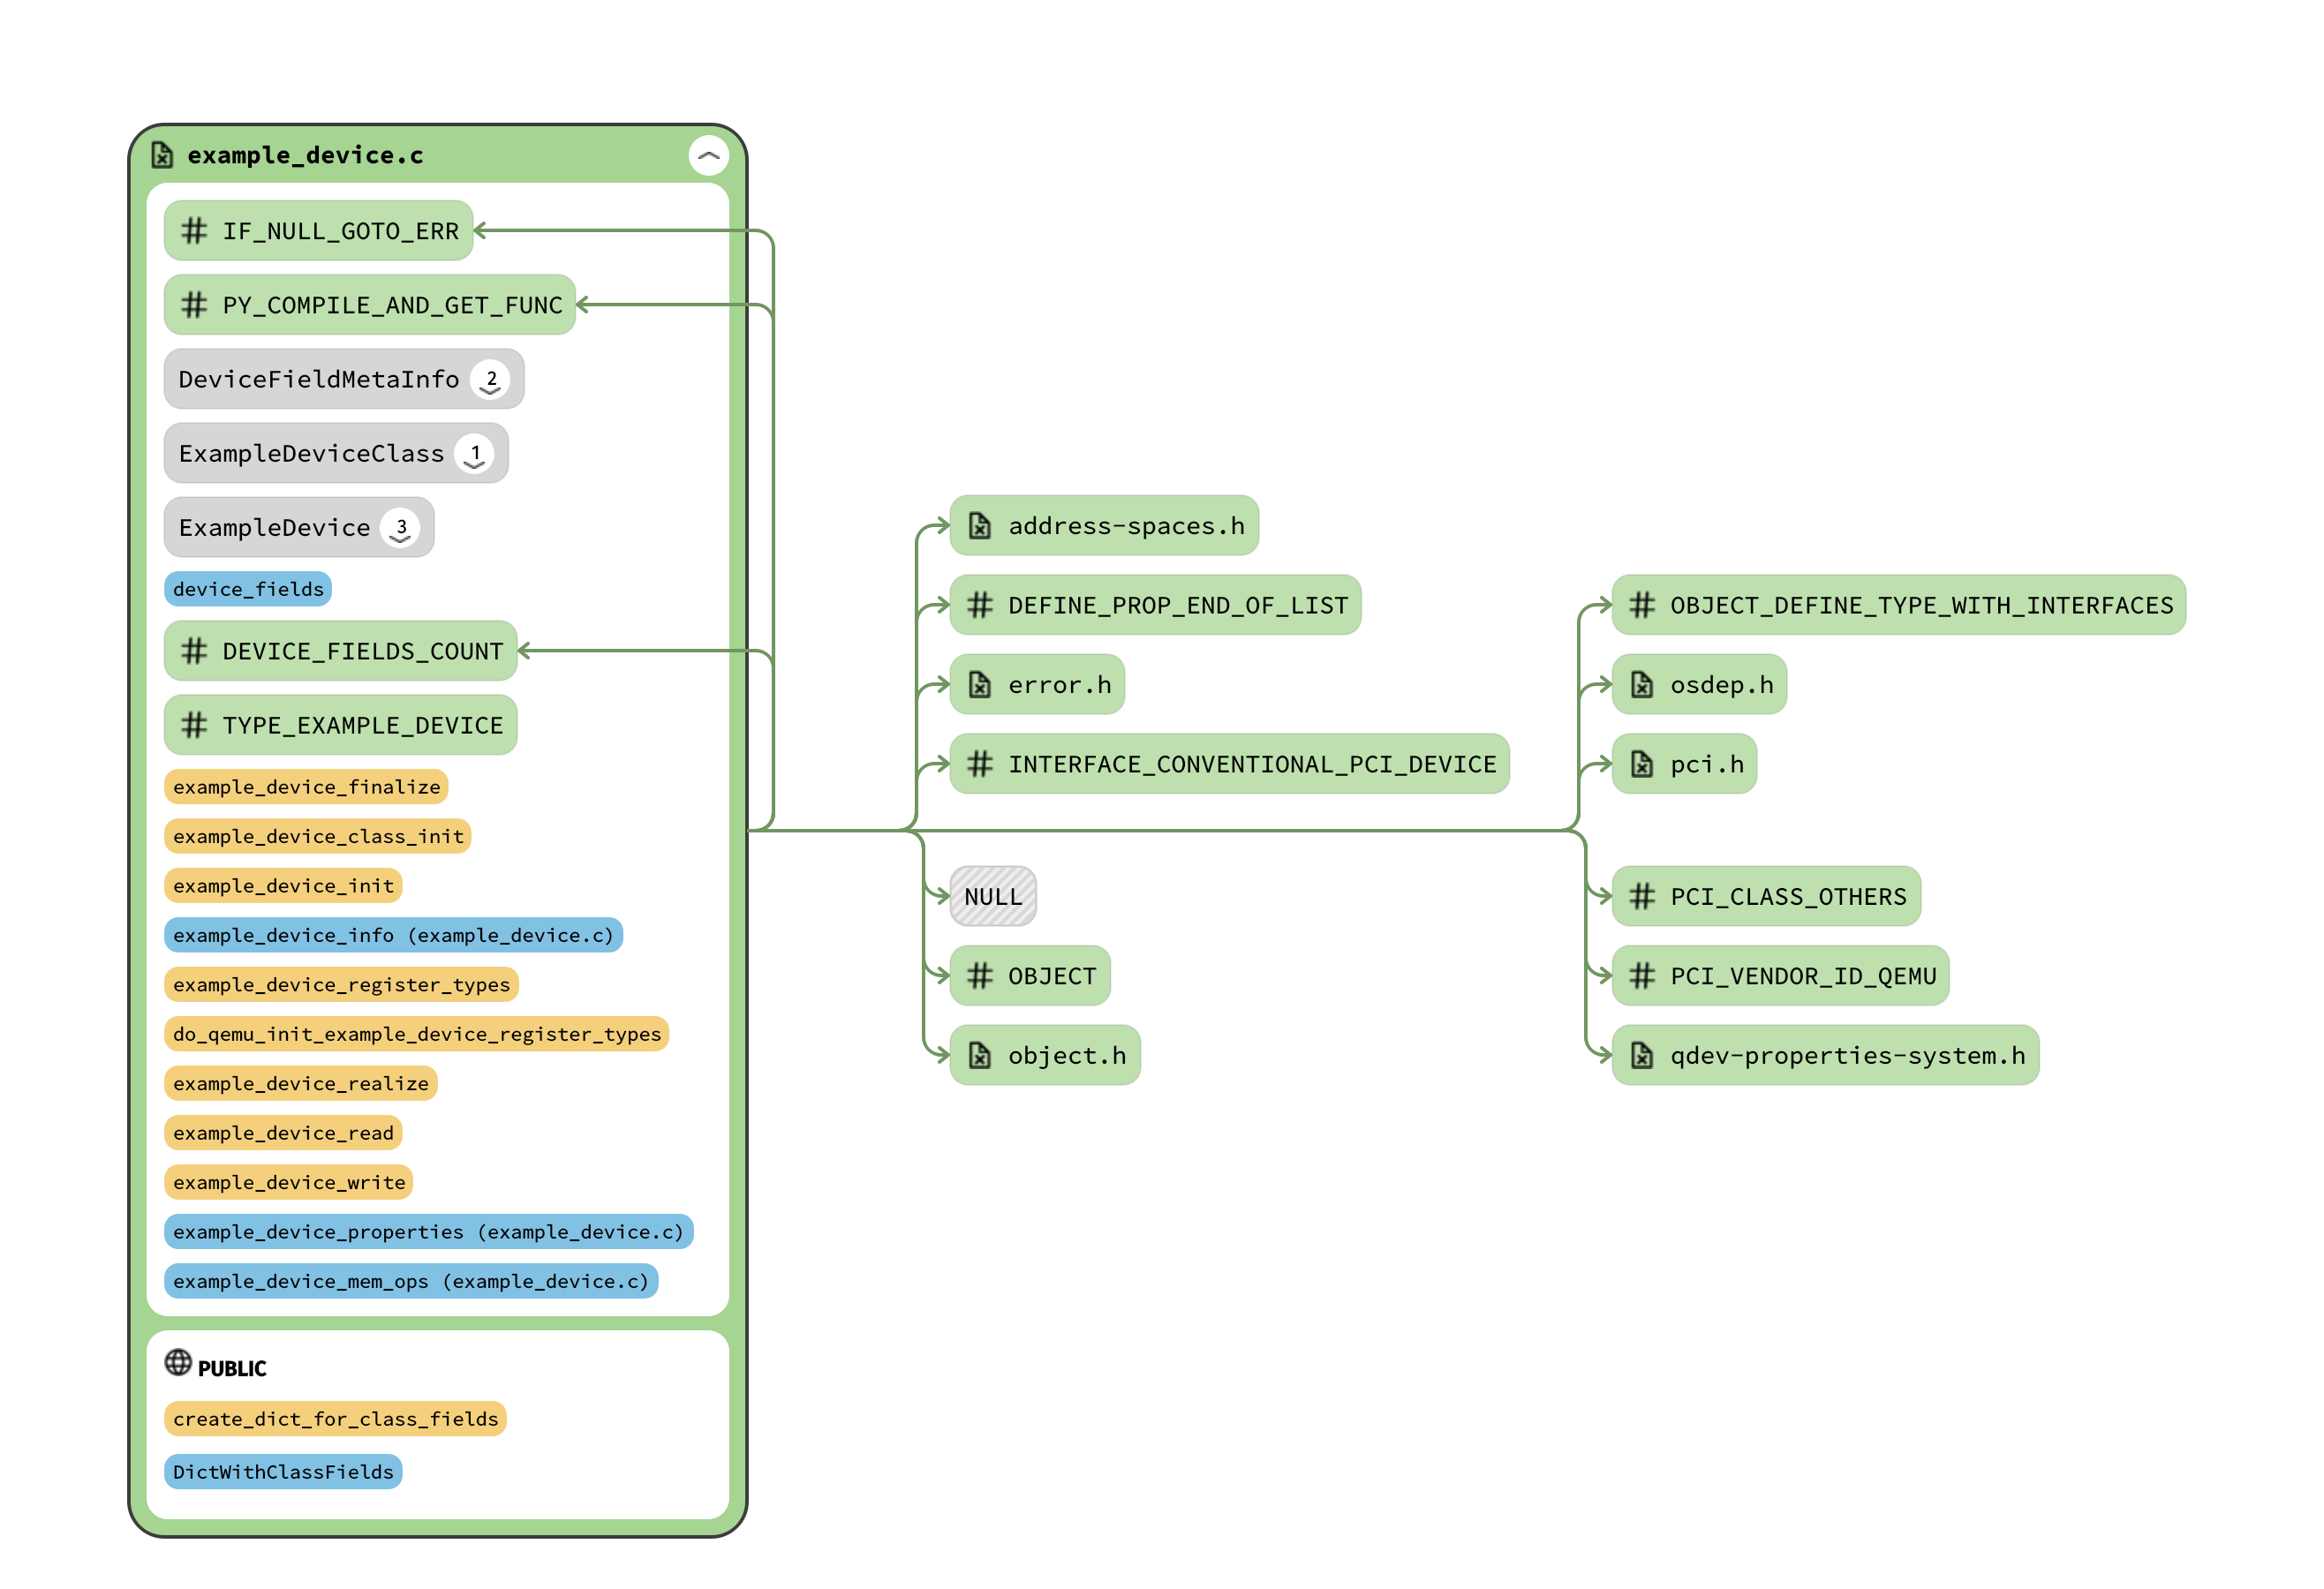
\includegraphics[]{images/experimental-device-class-diag.png}
        \end{adjustbox}
    \end{figure}
\end{frame}


\begin{frame}%[plain, noframenumbering, t]
    \frametitle{Выбор метрики оценки эффективности}
    Основные метрики эффективности разработанного языка:
    \begin{itemize}
        \item время разработки виртуального аппаратного обеспечения (в человеко-часах);
        \item быстродействие сгенерированного виртуального аппаратного обеспечения.
    \end{itemize}


    Экспериментальное устройство выполняет задачу сжатия JPEG-картинки.
    Данная задача легко поддается измерению, так как:
    \begin{itemize}
        \item легко выбрать сложность входных данных -- это
            размер изображения;
        \item возможна векторизация этапов алгоритма;
        \item возможно добавить разные подходы к обработке
            изображения:
            \begin{itemize}
                \item вызов подпрограммы;
                \item отправка данных по сети;
                \item реализация алгоритма устройства.
            \end{itemize}
    \end{itemize}
\end{frame}


\begin{frame}%[plain, noframenumbering, t]
    \frametitle{Оценка эффективности}
    \small
    \begin{longtable}{| p{2cm} | p{1.5cm} | p{1.5cm} | p{1.5cm} | p{1cm} |}
        \caption{Сравнение эффективности разработки и производительности виртуальных устройств реализующих
                 алгоритм сжатия JPEG картинки} \\
        \hline
            \multirow{2}{*}{Метрика} &
            \multicolumn{2}{c|}{Разработка с нуля} &
            \multicolumn{2}{c|}{Использование библиотеки} \\
        \cline{2-5} &
            C устройство &
            Python устройство &
            C устройство &
            Python устройство \\
        \hline
            Время разработки в человеко-часах &
            $100$ &
            $50$ &
            $35$ &
            $10$ \\
        \hline
            Время сжатия (сек.)&
            $3.915$ &
            $18.548$ &
            $1.871$ &
            $2.786$ \\
        \hline
    \end{longtable}
    {\small
        \textbf{Вывод:} разработка C-устройства дольше, и, соответственно, дороже,
        но преимуществом является быстрота его работы.
        Устройство, созданное {\mylanguage} сокращает время разработки вдвое.
        Использование библиотеки радикально сокращает
        время разработки в обоих случаях: в $2.8$ для C-устройства и
        $5$ раз для Python-устройства.
        При реализации устройств без сторонних библиотек, Python-устройство
        в $4.7$ раза медленнее аналогичного C-устройства. При использовании
        библиотек, разрыв сокращается до $1.5$ раза, что является
        более чем приемлемым.
    }
\end{frame}


\begin{frame}%[plain, noframenumbering, t]
    \frametitle{Основные результаты диссертационной работы}
    \begin{itemize}
        \item проведен аналитический обзор существующих методов создания виртуального аппаратного обеспечения;
        \item формализована задача создания виртуального аппаратного обеспечения;
        \item созданы методика и алгоритм генерации виртуального аппаратного обеспечения на основе его спецификации;
        \item разработан лингвистический аппарат (семантика, синтаксис) языка для создания программ по генерации виртуального
            аппаратного обеспечения;
        \item проведены эксперименты, результатом которых явилось сокращение времени разработки
            виртуального аппаратного обеспечения в $2$ раза по сравнению с классическим
            подходом, тогда как производительность устройства упала всего в $1.5$ раза.
    \end{itemize}
\end{frame}


\begin{frame}%[plain, noframenumbering, t]
    \begin{center}
        \Huge Спасибо за внимание!
    \end{center}
\end{frame}
